
\fancyhead[C]{Section 15.4}
\fancyhead[R]{\daysixteen}

\section*{\centering Chapter 15.4: Polar Coordinates}
\textbf{I3: Change of Variables.} I can use polar, cylindrical, and spherical coordinates to transform double and triple integrals and can sketch regions based on given polar, cylindrical, and spherical iterated integrals. I can use general change of variables to transform double and triple integrals for easier calculation.  I can choose the most appropriate coordinate system to evaluate a specific integral.

\subsection*{Mechanics}
\begin{enumerate}
\item \question{
        Use polar coordinates to compute the integral:
	\begin{equation*}
	\int_{0}^{2}\int_{-\sqrt{4-y^2}}^{\sqrt{4-y^2}} e^{-x^2-y^2} \ dx \ dy
	\end{equation*}
        }
        {% answer here
        
        }
        {% solution here
        
        }
    
	\item \question{
        Evaluate $\displaystyle \iint_D y^2+3x\ dA$ where $D$ is the region in the 3rd quadrant between $x^2+y^2=1$ and $x^2+y^2=9$.
        }
        {% answer here
        
        }
        {% solution here
        
        }
	
	\item \question{
        Use a double integral to determine the volume of the solid that is inside the cylinder $x^2+y^2=16$, below $z=2x^2+2y^2$, and above the $xy$-plane.
        }
        {% answer here
        
        }
        {% solution here
        
        }
    \item \question{
        Give an example of region and function you would \textit{not} want to use polar coordinates to integrate. Justify your answer. 
        }
        {% answer here
        
        }
        {% solution here
        
        }
\end{enumerate}
\subsection*{Applications}
\begin{enumerate}[resume]
    \item \question{
        The previous worksheet featured a problem involving a peculiar Pringles can. This problem rectifies that inconsistency.
    
    A true can of Pringles chips may be modeled by the cylinder $x^2+y^2=1$ bounded above and below like $0\leq z\leq 5$. Assuming that the Pringles container is filled up with chips until the surface $z=x^2-y^2+3$, are there more chips or air in the can? \textit{[Hint: Use the identity $\cos^2\theta-\sin^2\theta = \cos 2\theta$].}
        }
        {% answer here
        
        }
        {% solution here
        
        }
    
    \item \question{
        In the town of Churchill in northern Canada, the density of polar bears around the town dump is given by $p(x,y)=e^{x^2+y^2}$ bears per square unit. Use polar coordinates to compute the average number of polar bears in the region $1\leq x^2+y^2\leq 2 $.
        }
        {% answer here
        
        }
        {% solution here
        
        }
\end{enumerate}
\clearpage

\subsection*{Extensions}
\begin{enumerate}[resume]	
	\item \question{
        Find the area of the region common to the interiors of the cardioids $r=1+\cos \theta$ and $r=1-\cos \theta$. \textit{[Hint: Use symmetry to restrict your calculation to only the first quadrant.]}
	
	\begin{center}
		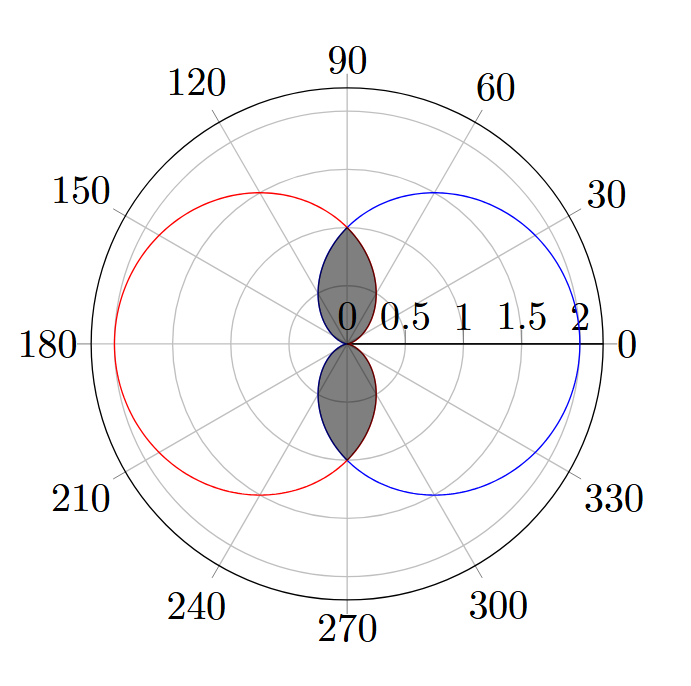
\includegraphics[scale=0.4,alt={plot of the double-teardrop shaped region between the two cardioids specified above, with intersection points at (r,theta)=(0,0),(1,pi/2),(1,3pi/2)}]{ws_15_4_cardioids.png}
	\end{center}
        }
        {% answer here
        
        }
        {% solution here
        
        }
	
	\item \question{
        An integral of great importance in statistics is the Gaussian integral $I=\Ds \int_0^\infty e^{-x^2}\ dx$.  The function $f(x)=e^{-x^2}$ has no elementary antiderivative, so this integral is hard to compute in the usual way. Fortunately, polar coordinates provide a solution.
	
	Notice that $I^2=\Ds \left(\int_0^\infty e^{-x^2}\ dx\right)\left(\int_0^\infty e^{-y^2}\ dy\right) = \int_0^\infty \int_0^\infty e^{-x^2-y^2}\ dxdy $.
	
	\begin{enumerate}
		\item The domain of the above double integral is the first quadrant $[0,\infty)\times [0,\infty)$. Describe this region using polar coordinates, and transform $I^2$ into an (improper) polar integral. 
		
		\item Evaluate your double integral to compute the value of $I^2$.  Use this to find the value of the original Gaussian integral $I$.
	\end{enumerate}

	You can find some history of this integral \href{https://www.york.ac.uk/depts/maths/histstat/normal_history.pdf}{here}.
        }
        {% answer here
        
        }
        {% solution here
        
        }
	
\end{enumerate}
{}

\iftoggle{answers}{
\begin{center}{\large \textbf{Math 2551 Worksheet Answers: Polar Double Integrals}}
\end{center}

\begin{enumerate}
	\item $5\pi-26$
	
	\item $\dfrac{\pi}{2}(1-e^{-4}).$
	
	\item $\dfrac{3\pi}{2}-4$.
	
	\item $256\pi$
	
	\item \begin{enumerate}
		\item $I^2=\Ds \lim_{R\to\infty}\int_0^2\pi\int_0^R e^{-r^2}r\ dr\ d\theta$
		
		\item $I^2=\dfrac{\pi}{4}$, so $I=\dfrac{\sqrt{\pi}}{2}$
	\end{enumerate}
\end{enumerate}
}{}
\iftoggle{solutions}
{
Solutions go here in the same format.
}{}